\chapter{Results}\label{sec:results}

The geological map of the study area \parencite{Linth_Map} provides a classification for 
all sample locations. Samples mapped as \USM are classified as freshwater,
\UMM as marine~(cf. fig.~\ref{fig:study_area}). The flysch and \OSM samples are marine and 
freshwater respectively \parencite{Linth_Text,gubler_2009e}. 

The XRF instrument reports the \emph{Compton ratio} as an indicator for the reproducibility,
and thus reliability, of the measurements. For most samples the instrument reports moderate to low 
Compton ratios (\cref{tab:sr-ba-table}), 
suggesting that the results should be interpreted only qualitatively.
Quantitative interpretation should be approached with caution.

\section{Cl/Br}

The \XRF measurements for \acro{Cl} were inconsistent. \acro{Cl} was detected in only six samples,
and only one sample yielded \acro{Cl} in both pellets. 
\acro{Br} was not detected in any sample. 

The \ICPMS measurements of halogens following the \ambif\ method of \textcite{he_determination_2019}
produced inconsistent results. Throughout the measurement cycle, instrument sensitivity
decreased by approximately two orders of magnitude (\cref{fig:halogen-sensitivity}).

When the raw \acro{Cl} counts of the standard solutions are plotted
against the respective concentrations of 10, 100 and 1000\,ppb Cl, the linear regression line does not
pass through (0,0), instead it shows a large positive intercept. Subtracting the regression intercept
from the measured counts, the \acro{Cl} counts are comparable to \acro{Br}~(\cref{fig:cl-br-counts-run1}).
The reagent blanks containing only \ambif\ also show high Cl counts~(\cref{fig:cl-br-blanks}).
This indicates a systematic background signal for Cl.

\acro{Cl} (after correction) and \acro{Br} showed different results across the three standard solutions
of 10, 100 and 1000\,ppb Cl and Br throughout the measurement run~(\cref{fig:cl-br-counts}).
At the beginning, the counts for \acro{Br} increased linearly with concentration as expected, 
while the trend for \acro{Cl} was not quite as clear~(\cref{fig:cl-br-counts-run1}).
At the end of the measurement run, after all samples had been measured, \acro{Br} still displayed a clear linear
increase, while \acro{Cl} appeared more scattered and showed no linear trend~\Cref{fig:cl-br-counts-run3}.

We observed significant instrument corrosion after the measurements and attribute the
decline in instrument sensitivity to this damage. 
Therefore, the results cannot be considered reliable, and will not be discussed further.

\begin{figure}[]
  \nopagebreak
  % Left side: The Figure
  \begin{minipage}[t]{0.48\textwidth}
    \vspace{0pt}
    \centering
    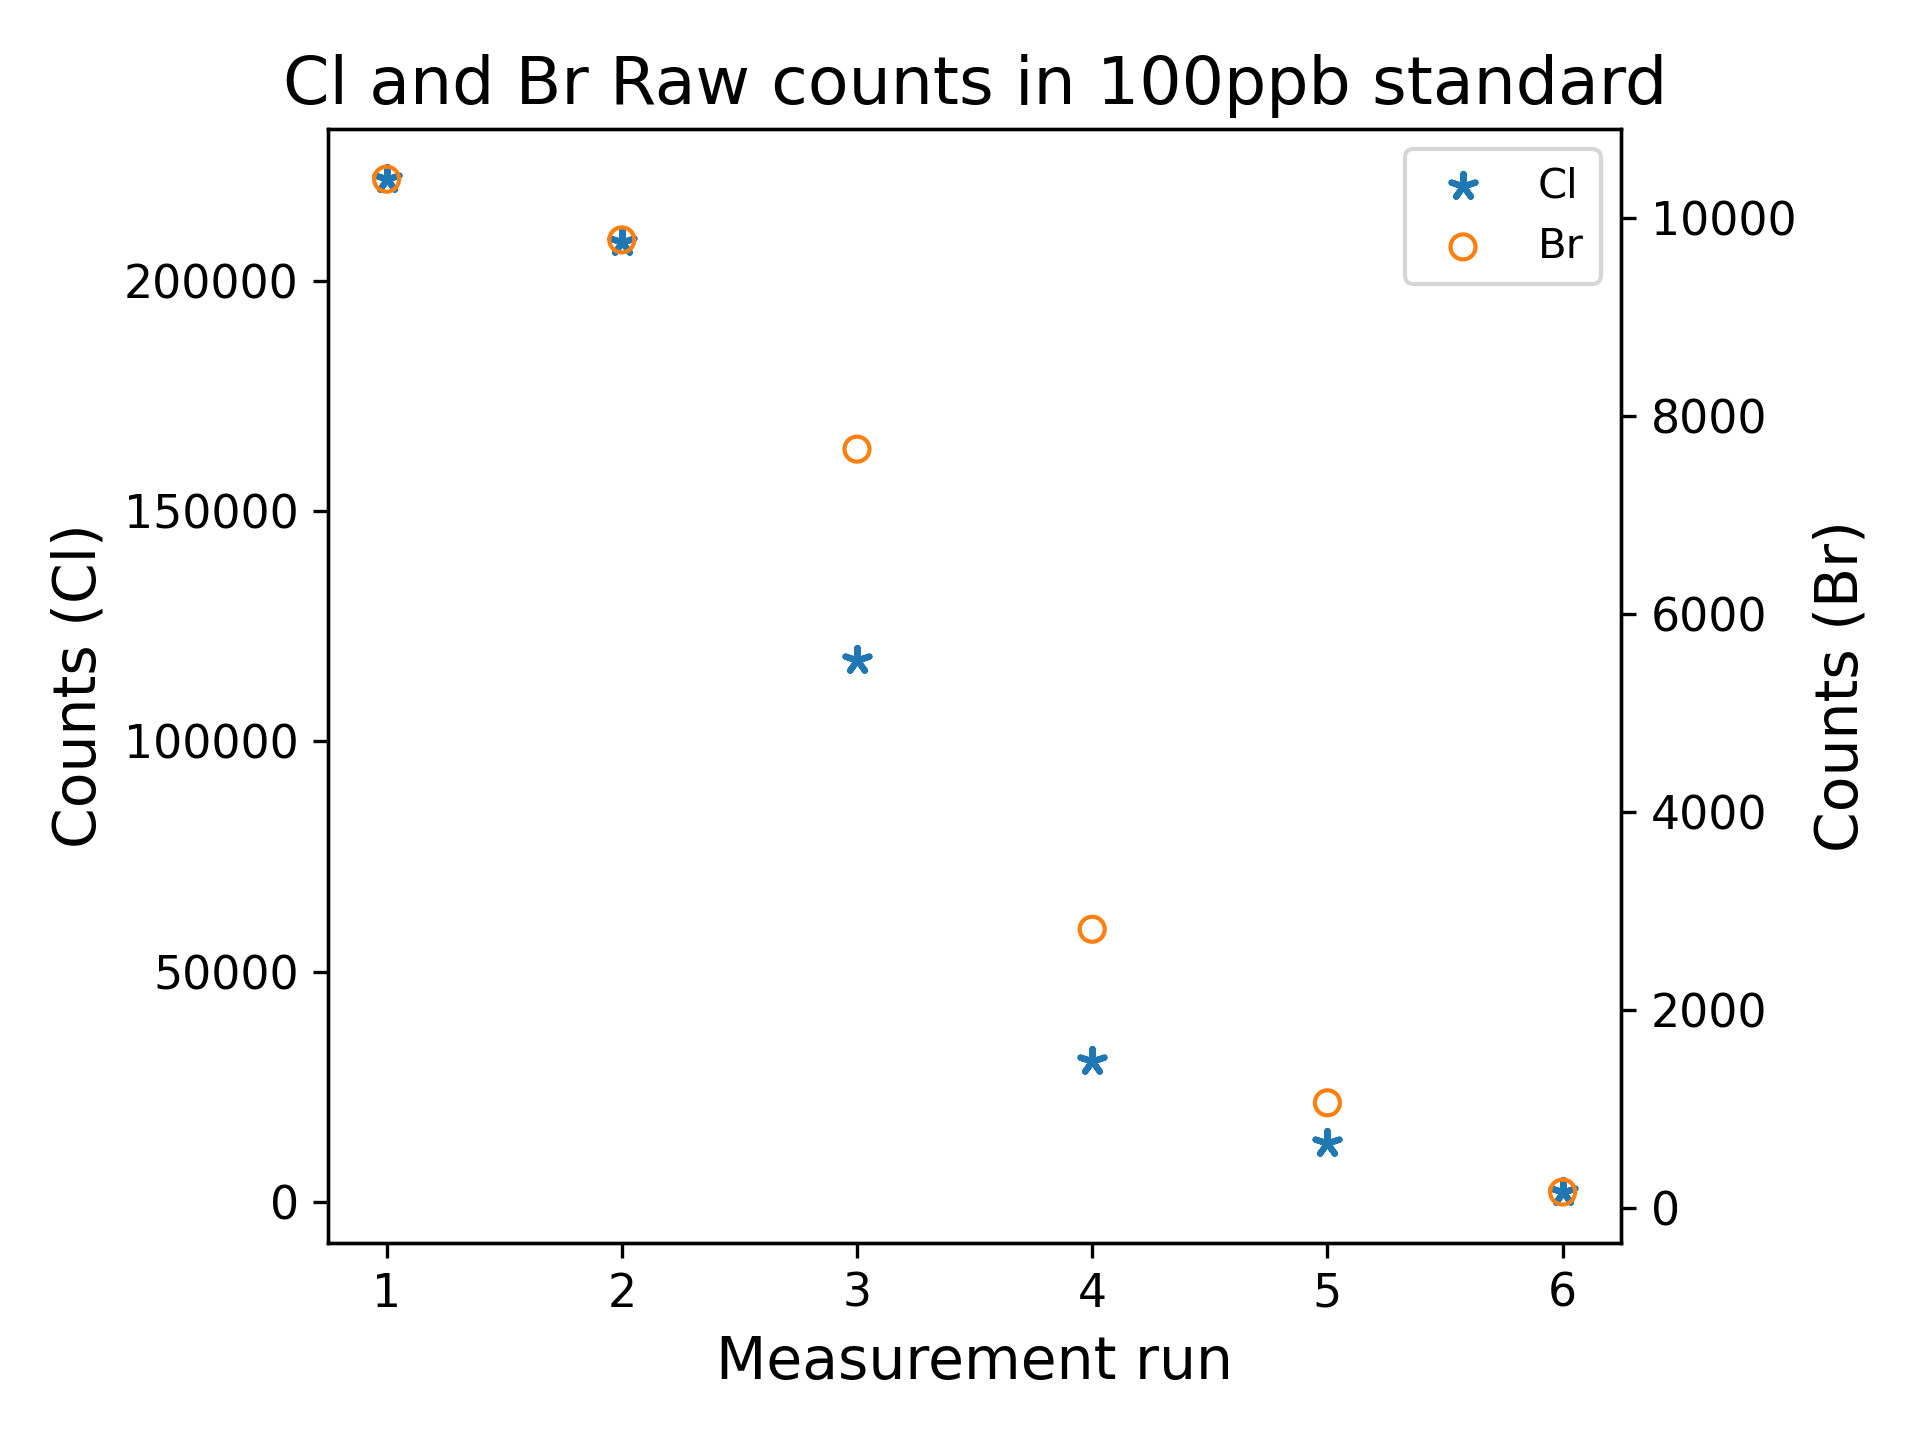
\includegraphics[scale=0.47]{img/icpms_halogen_sensitivity.png}
    \captionsetup{width=0.95\linewidth}
    \caption{Counts for Cl and Br throughout the measurement run. The measured solution
    is always with 100\,ppb Cl and Br.}
    \label{fig:halogen-sensitivity}
  \end{minipage}
  \hfill % Adds horizontal space between the minipages
  % Right side: The Table
  \begin{minipage}[t]{0.48\textwidth}
    \vspace{0pt}
    \centering
    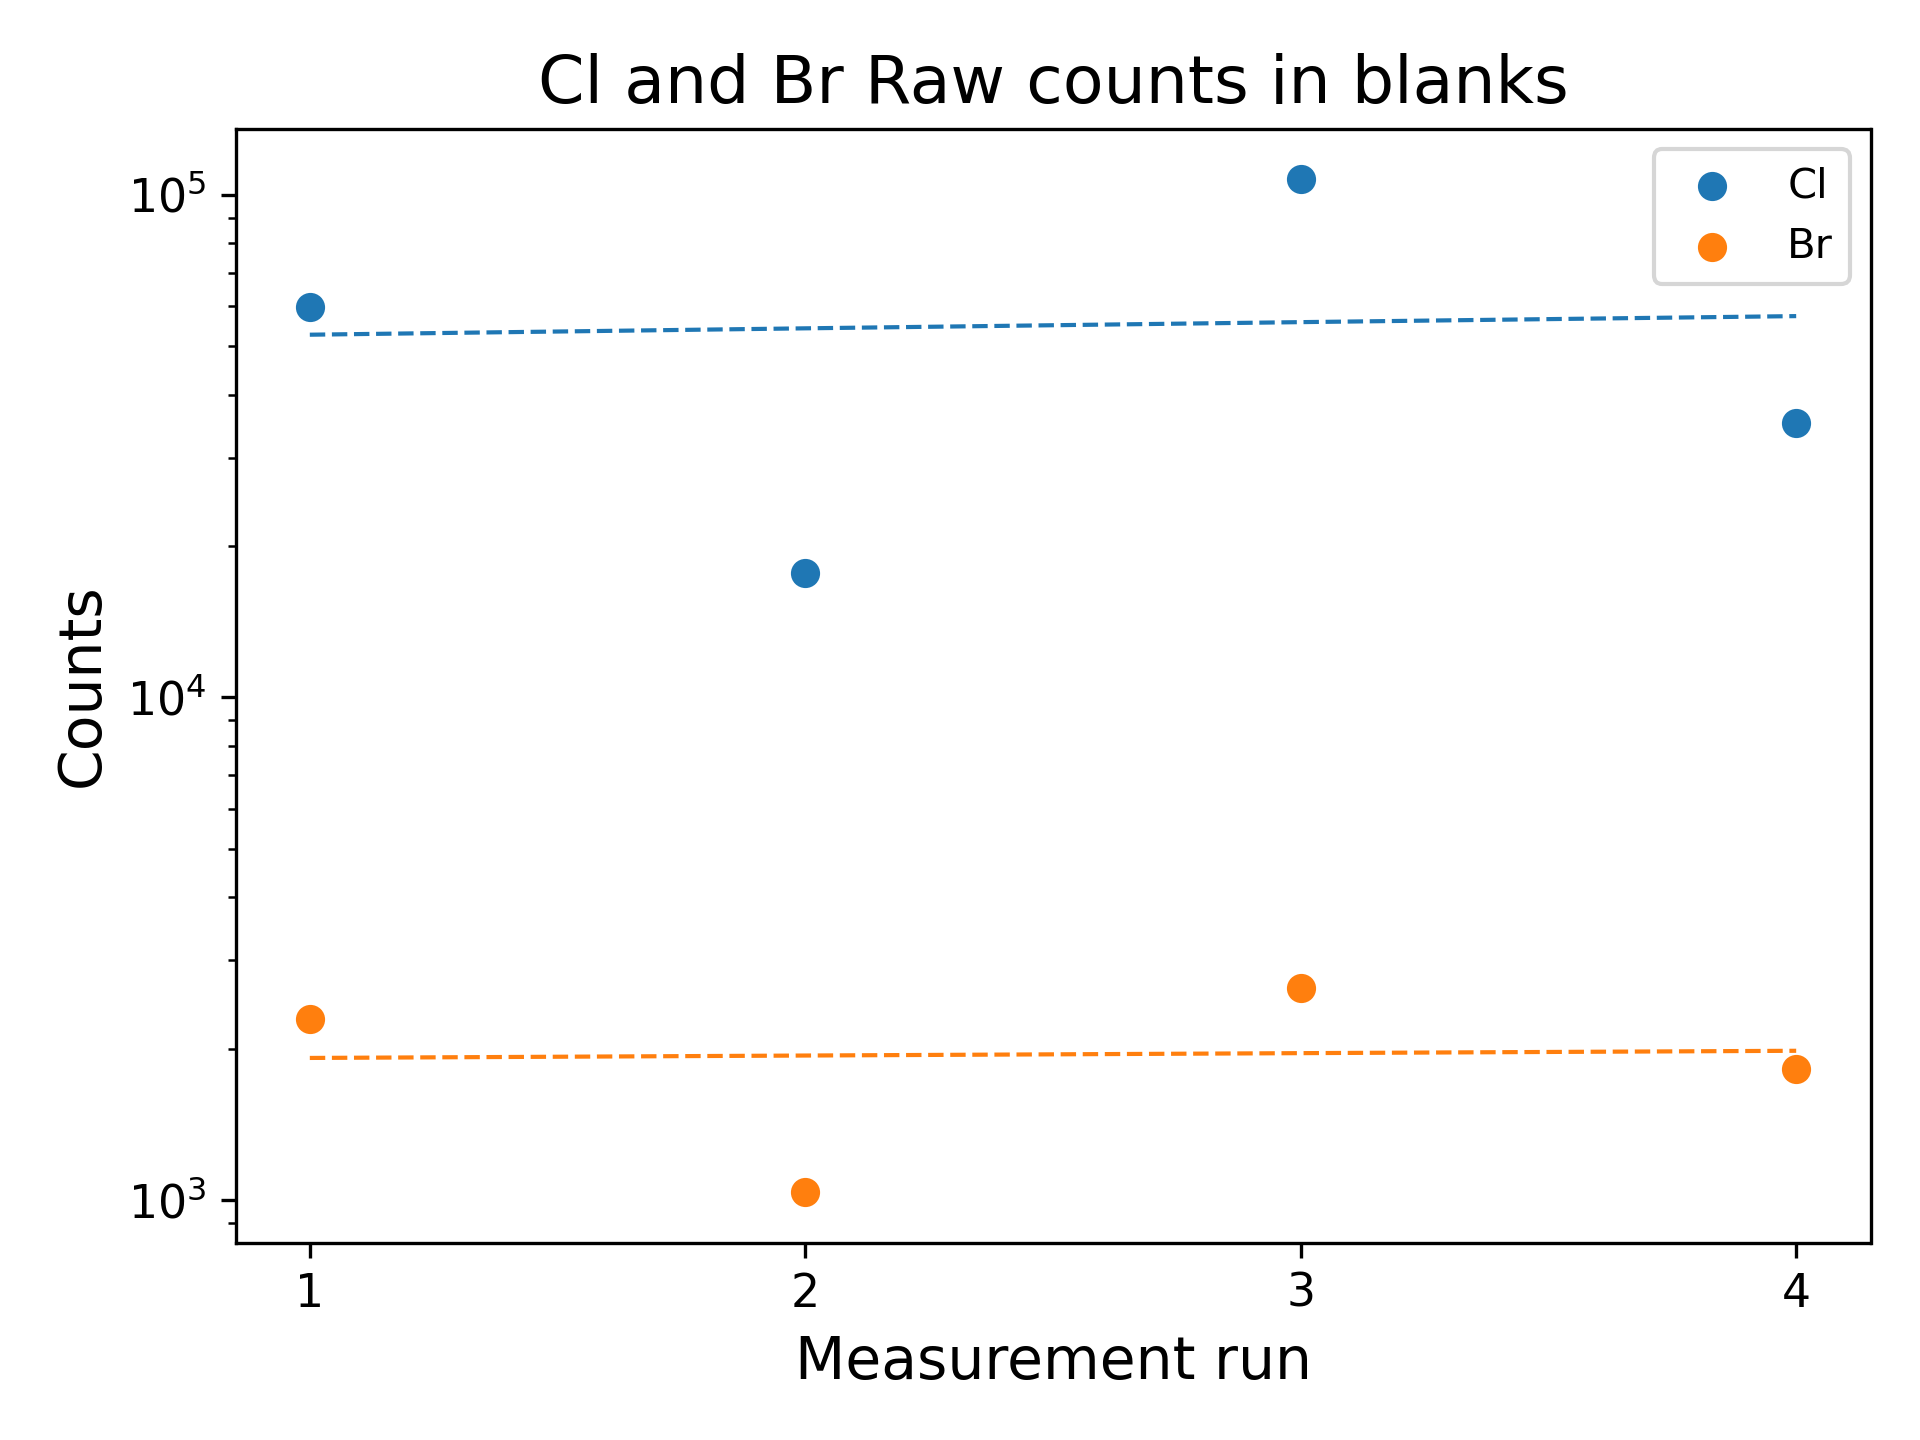
\includegraphics[scale=0.47]{img/cl_br_blanks.png}
    \captionsetup{width=0.95\linewidth}
    \caption{Measurement of \ambif\ reagent blanks show that Cl counts are systematically higher than Br.}
    \label{fig:cl-br-blanks}
  \end{minipage}
\end{figure}


\section{Sr/Ba}

\XRF yielded \acro{Sr} and \acro{Ba} concentrations for all samples except for the \OSM
reference sample, in which no \acro{Ba} was detected.
The \acro{Ba} measurements had uncertainties of approximately 10\%, while
the uncertainties for \acro{Sr} were approximately 0.5\% (\cref{tab:sr-ba-table}).
\ICPMS yielded \acro{Sr} and \acro{Ba} concentrations for all samples. 
Compared to \XRF, the \ICPMS concentrations for \acro{Ba} were approximately 50\% lower,
while \acro{Sr} was typically
50-100\,ppm higher. The uncertainties were 13.7\% for \acro{Ba} and 7\% for \acro{Sr}~(\cref{tab:sr-ba-icpms-table}).

\Cref{fig:sr_ba_crossplot} shows \acro{Sr} over \acro{Ba} for both methods.
The data points are colour-coded based on the classification in \parencite[\protect\cref{fig:study_area}]{Linth_Map}.
This classification
corresponds to \emph{marine} for \UMM and Flysch, and \emph{freshwater} for \USM and \OSM.
This classification highlights JWL 1 as an outlier compared to the other freshwater samples.

\begin{figure}
    \centering
    \subfigure[Standard Cl and Br counts \emph{before} measuring samples.\label{fig:cl-br-counts-run1}]{
        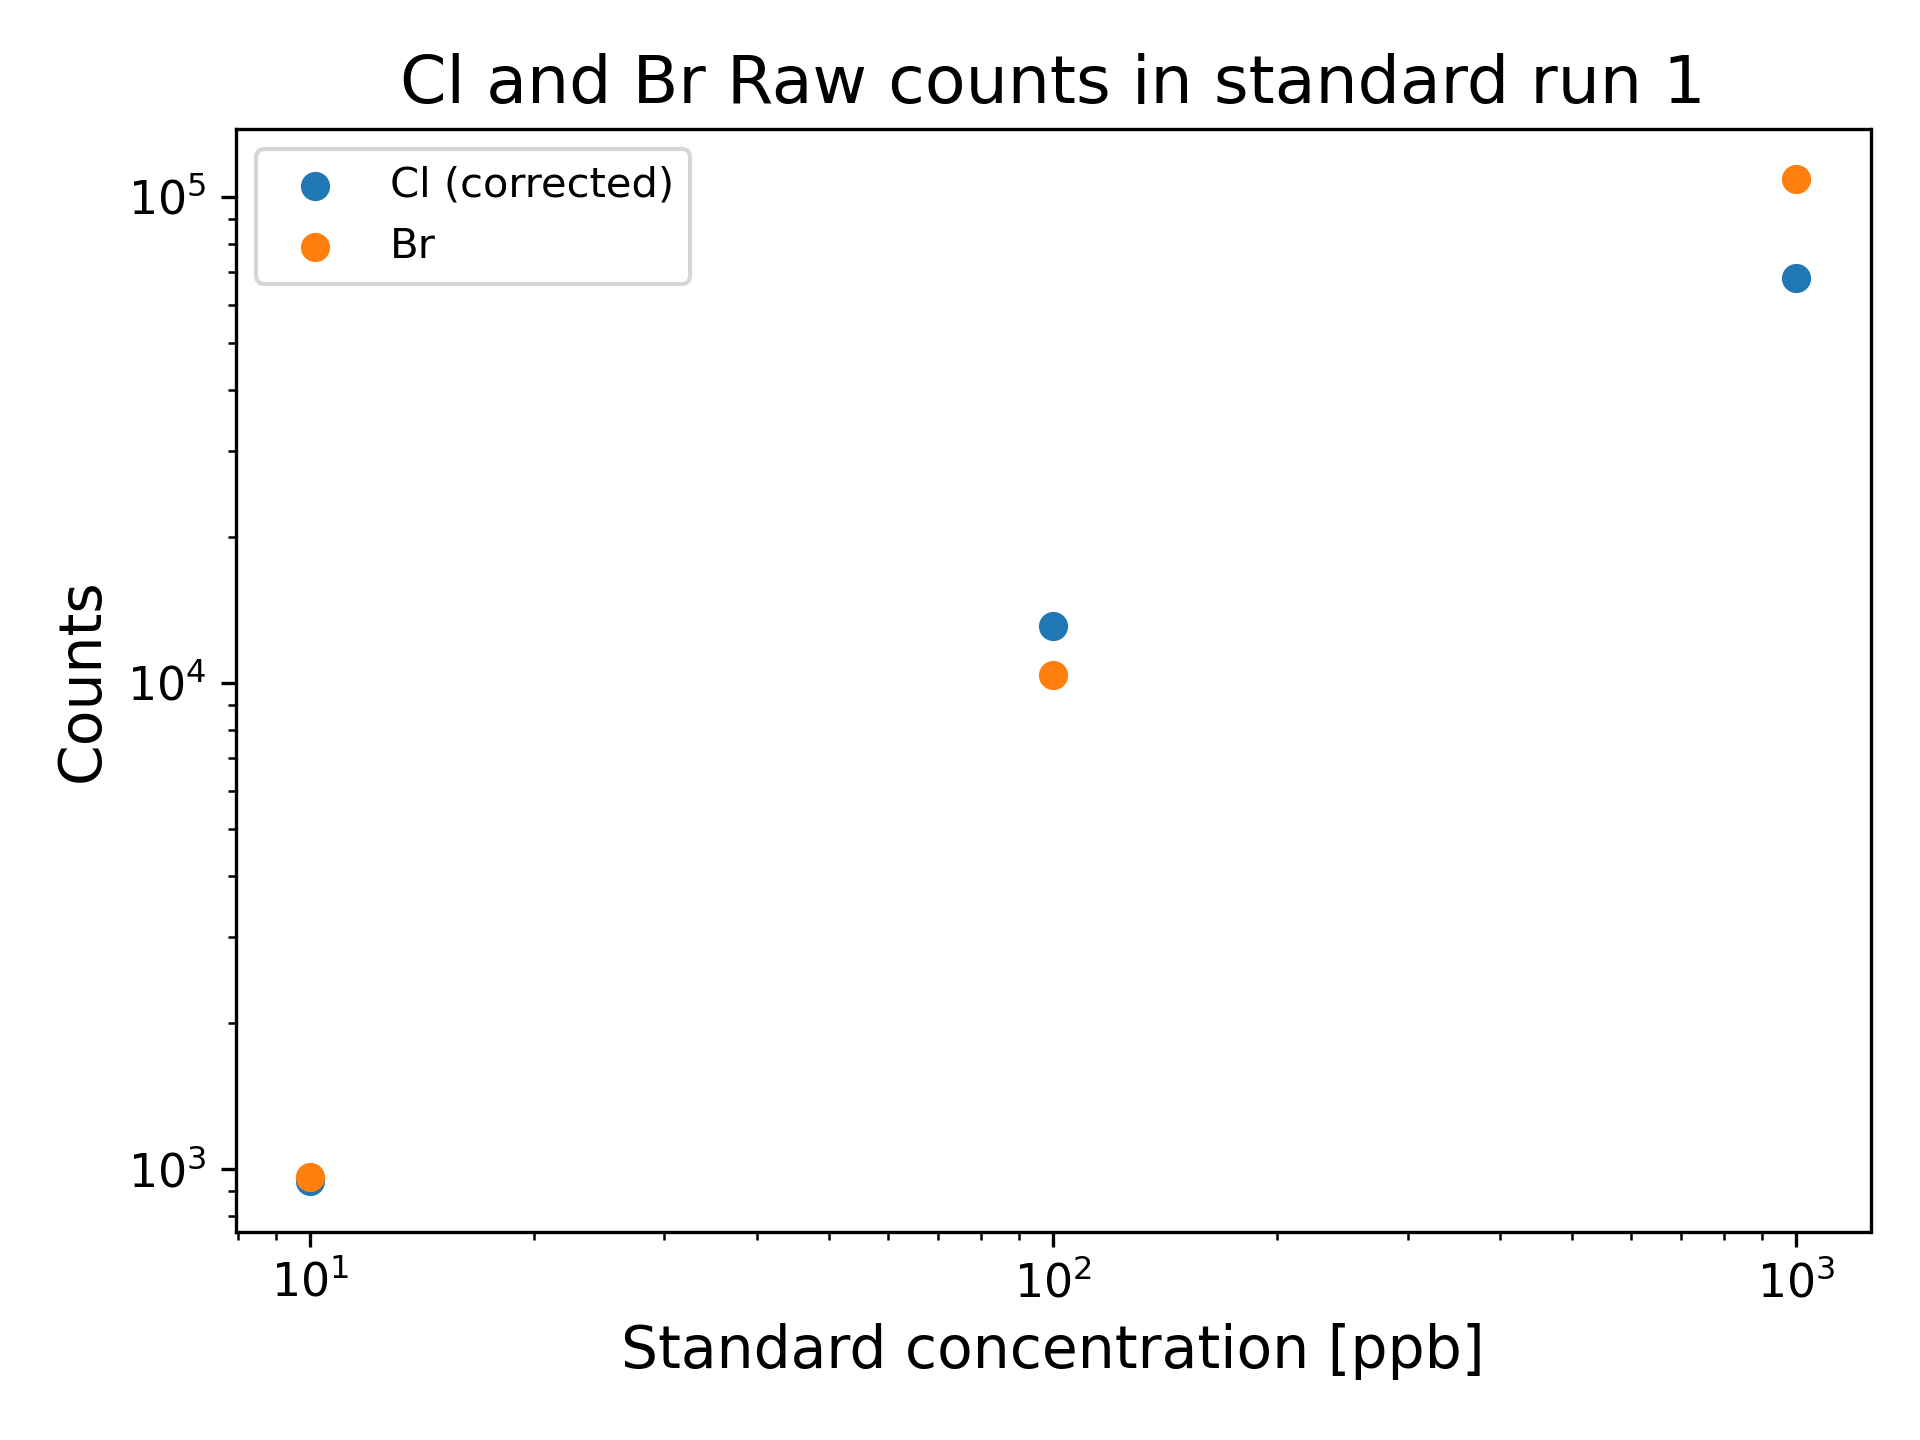
\includegraphics[width=0.45\textwidth]{img/cl_br_standards_run1.png}}\qquad
    \subfigure[Standard Cl and Br counts \emph{after} measuring samples.\label{fig:cl-br-counts-run3}]{
        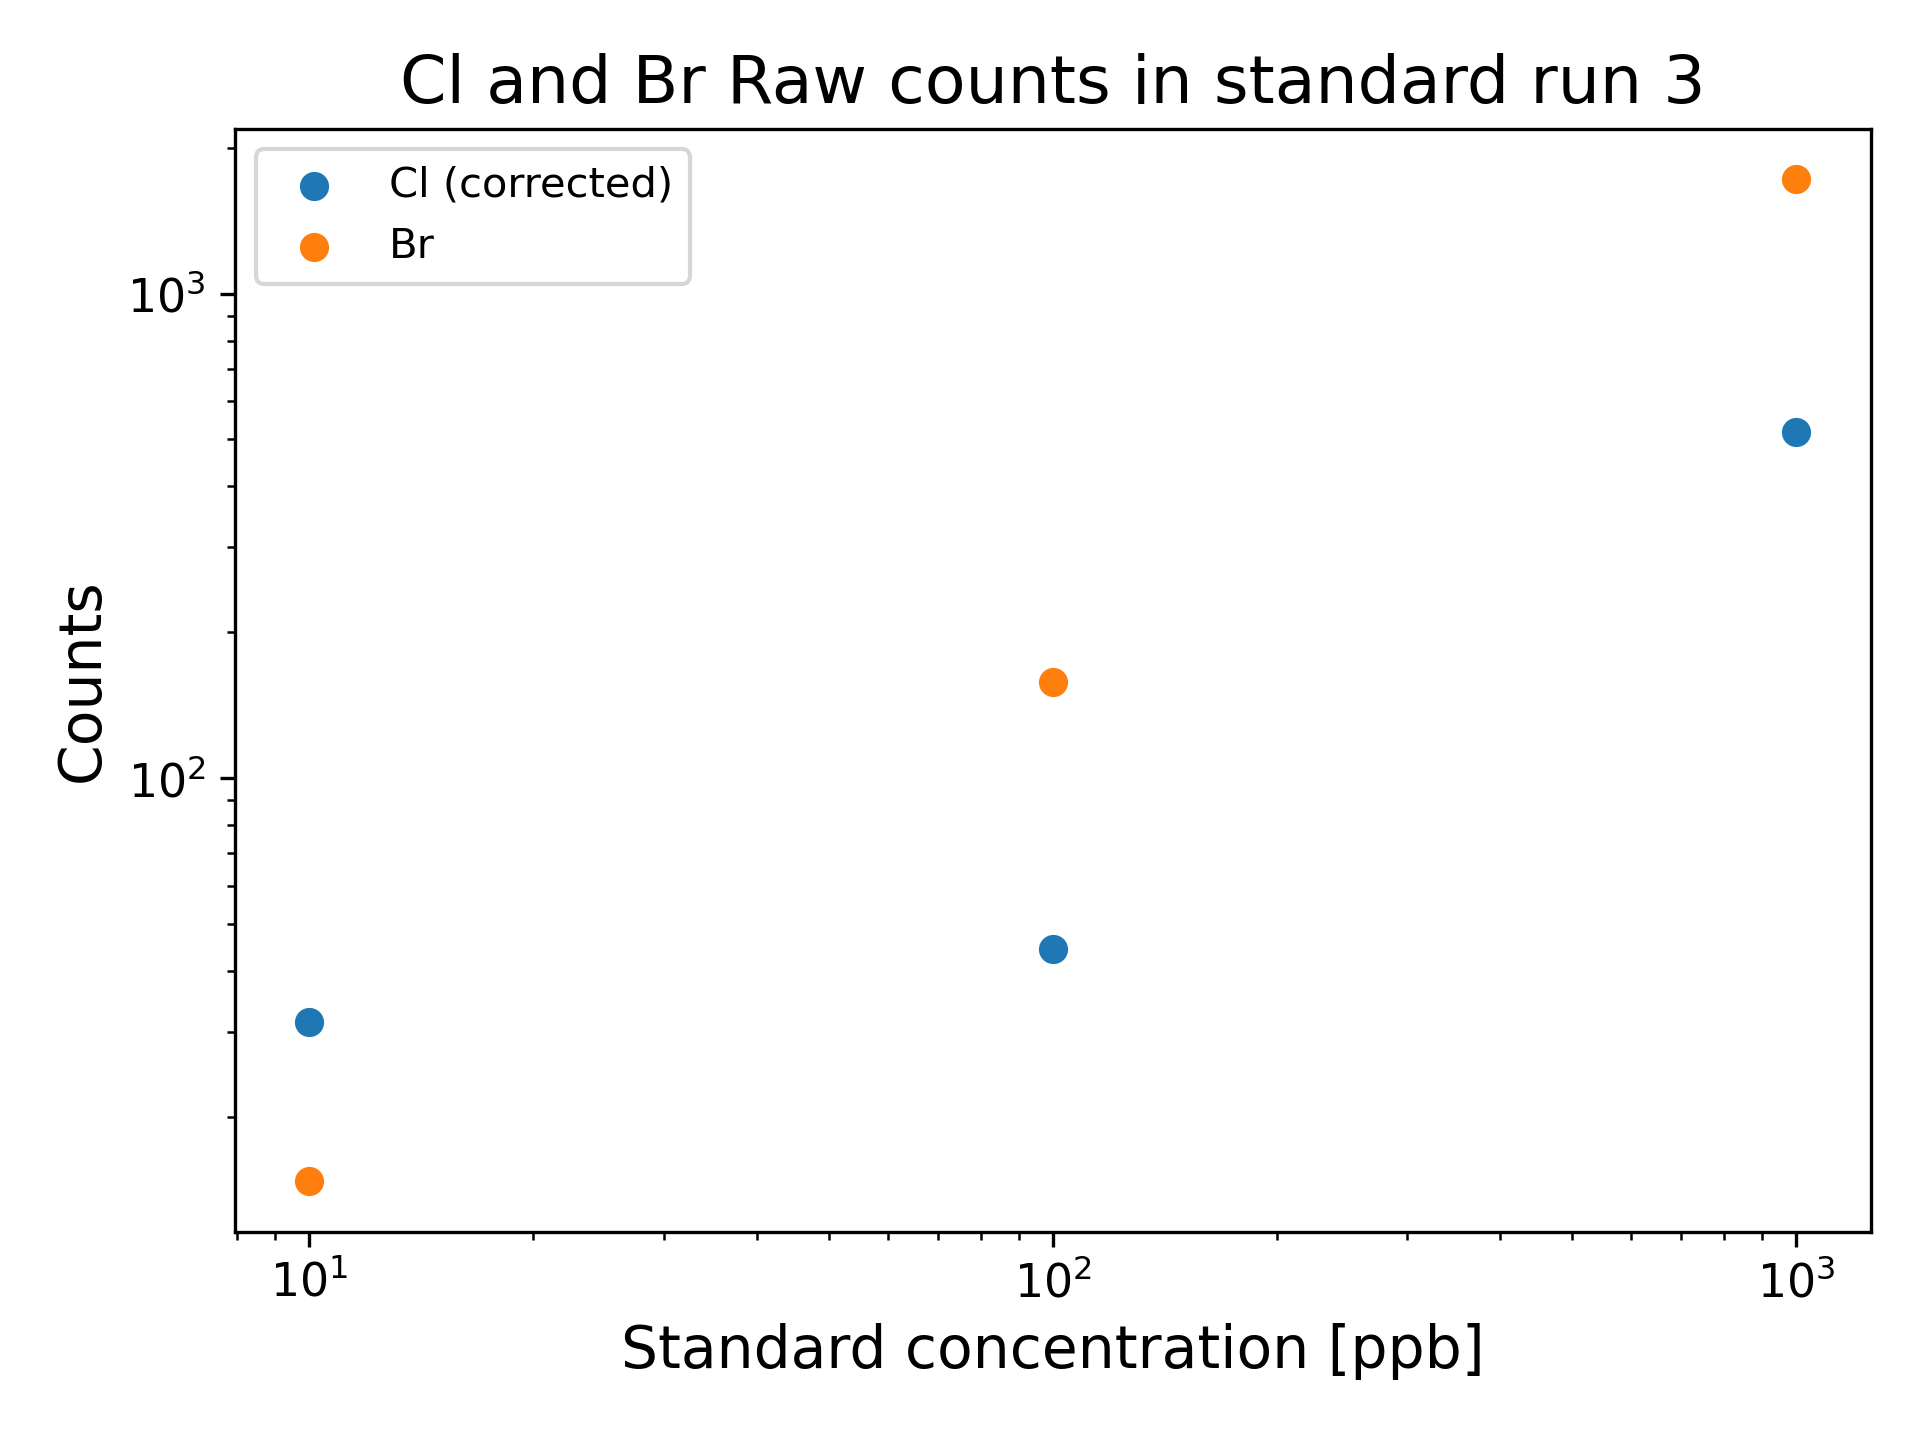
\includegraphics[width=0.45\textwidth]{img/cl_br_standards_run3.png}}
    \caption{Cl (after correction) and Br show the expected linear dependence on
    solution concentrations at the beginning of the measurement (run 1), but
    Cl is not linear in the final run 3.}
    \label{fig:cl-br-counts}
\end{figure}

\textcite{wei-2020} determined Sr/Ba ratios of 0.5 and 0.2 as thresholds between marine/brackish and 
brackish/freshwater. These ratios are plotted as light grey lines. Third, the ROC curve best fit ratio
is plotted the red lines. The best fit lines are corrected for the outlier JWL 1. 
The plots for both measurement methods show that the data do not fit the model from \textcite{wei-2020}.

\section{S/TOC}

\acro{IRMS} yielded \TOC measurements for all samples, but no uncertainties were determined.
\XRF and \ICPMS consistently measured \acro{S} for all samples~(\cref{tab:s-toc-table,tab:s-toc-icpms-table}).
For XRF, we obtained results for two pellets for each sample and standard, whereas only one \TOC result
was available for each. Therefore, to match measurements for S from XRF with \TOC, we averaged the S results
of the two pellets per sample.

\Cref{fig:toc_s_crossplot} shows cross-plots of \acro{S} over \TOC. The plot layout is 
similar to that for Sr/Ba (\cref{fig:sr_ba_crossplot}), but the brackish/freshwater threshold is 
0.1 instead of 0.2. Additionally, it shows the normal trend for S/TOC in marine settings
from \textcite{berner-raiswell-1983}. The normal freshwater trend, also proposed by these authors, coincides 
with the brackish threshold of \textcite{wei-2020}, therefore it is not plotted separately.

\begin{figure}
    \centering
    \includegraphics*[width=0.95\textwidth]{img/sr_ba_combined.png}
    \caption{Sr/Ba data from XRF (left) and \ICPMS (right). 
    The colour coding into marine (UMM/Flysch) and freshwater (USM/OSM) is
    based on the classification of the sample locations in \textcite{Linth_Map}. 
    The grey lines are the dividers given by \textcite{wei-2020},
    the red line is a best fit for our data.
    }\label{fig:sr_ba_crossplot}    
\end{figure}

The most notable difference between the \XRF and \ICPMS data is the \acro{S} concentration for 
marine samples.
\ICPMS reported concentrations approximately twice as high as those from \XRF, 
while the freshwater samples showed roughly the same concentrations
with both methods. Because \TOC was determined independently and only once,
the x-axis is identical in both plots. 

Despite the differences, both datasets show that marine and freshwater samples group in two 
distinct clusters.
The freshwater samples fall 
into the freshwater sector proposed by \textcite{wei-2020} and close to the general
freshwater trend of \textcite{berner-raiswell-1983}. The marine samples fall
into the brackish sector, and in the case of the \XRF data, much closer to the freshwater trend 
than to the marine trend of \textcite{berner-raiswell-1983}. JWL 1 is an exception in all cases
and shows a strong marine signal.

With the XRF data, the fitted threshold falls below the normal freshwater trend
from \textcite{berner-raiswell-1983}, and all data points are close to that threshold. 
With \ICPMS, the fitted threshold falls between the marine and freshwater
trends.


\section{Carbonate}

Carbonates can influence the Sr content in sedimentary rocks significantly~\parencite{wei-2020}.
To estimate the upper bound on carbonate content in our samples, we attributed all Ca (measured with \ICPMS)
to CaCO$_3$ (\cref{fig:carbonate}). 

This estimate is reasonable, because the main Ca-bearing minerals in rocks are carbonates,
feldspars, pyroxenes and evaporites. In fine-grained detrital sediments in marginal settings, like those in our 
case study, most of these minerals have undergone chemical weathering and are either fully dissolved or
have been altered to clays, which contain little Ca in their crystal structure. Ca may adsorb to
clays, which is why our estimates represent upper bounds to carbonate.

\begin{figure}
    \centering
    \includegraphics*[width=0.95\textwidth]{img/toc_s_combined.png}
    \caption{S data from XRF(left) and \ICPMS(right), TOC from IRMS. 
    The colour coding into marine (UMM/Flysch) and freshwater (USM/OSM) is
    based on the classification of the sample locations in \textcite{Linth_Map}. 
    The light grey lines are the dividers given by \textcite{wei-2020}, the dark grey line
    is the normal marine trend for S/TOC from
    \textcite{berner-raiswell-1983}, the red line is a best fit for our data.
    }\label{fig:toc_s_crossplot}    
\end{figure}

\begin{figure}[b]
    \centering
    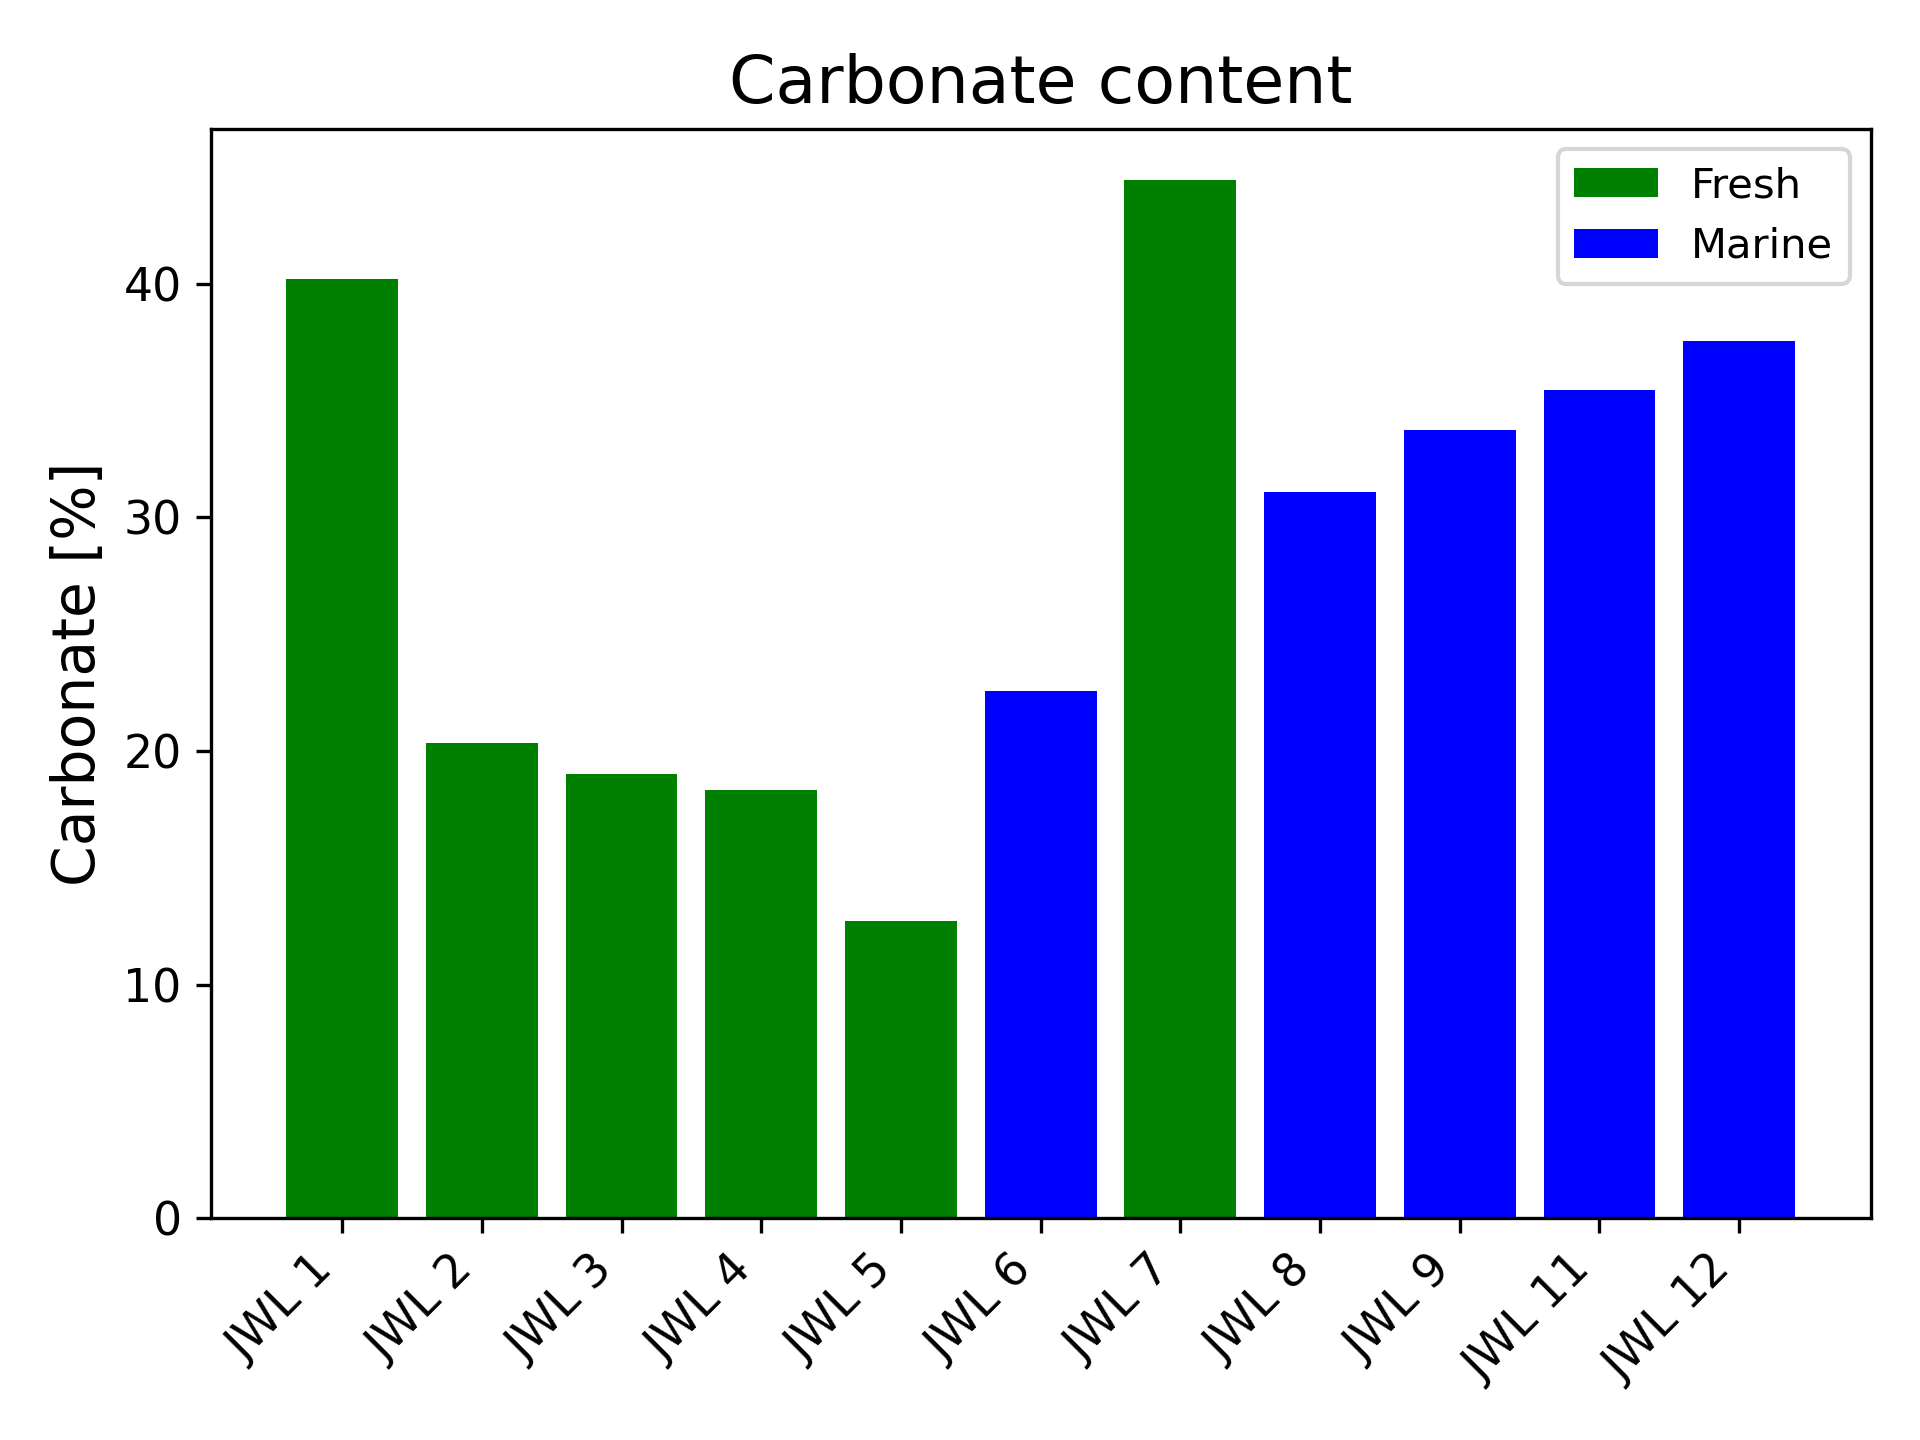
\includegraphics[width=.4\textwidth]{img/icpms_carbonate.png}
    \caption{Upper bounds on carbonate content in the samples estimated from Ca measurements with \ICPMS,
    attributing all measured Ca to CaCO$_3$.}
    \label{fig:carbonate}
\end{figure}